\section{Testy i~walidacja systemu}
\label{chap:testy}

Rozdział przedstawia wyniki testów systemu RiskScoop AI. Przeprowadzono testy funkcjonalne, testy wydajnościowe oraz testy interpretacji języka naturalnego.

\subsection{Metodologia testów}

\subsubsection{Środowisko testowe}

Testy przeprowadzono w~następującym środowisku:
\begin{itemize}
    \item komputer: MacBook Pro M2 Pro, 16GB RAM,
    \item system operacyjny: macOS 15.1,
    \item backend: Python 3.12, Agno AgentOS, Gemini 3 Pro,
    \item frontend: Vanilla JS, Mapbox GL JS v3.0,
    \item baza danych: MotherDuck (DuckDB w~chmurze),
    \item sieć: łącze 300 Mbps (Wi-Fi 6).
\end{itemize}

\subsubsection{Zakres testów}

Testy obejmowały:
\begin{enumerate}
    \item \textbf{testy funkcjonalne} -- weryfikacja poprawności działania wszystkich narzędzi,
    \item \textbf{testy interpretacji NL} -- ocena poprawności rozumienia zapytań w~języku naturalnym,
    \item \textbf{testy wydajnościowe} -- pomiar czasów odpowiedzi poszczególnych narzędzi.
\end{enumerate}

\subsection{Testy funkcjonalne}

\subsubsection{Scenariusze testowe}

Przeprowadzono 15 scenariuszy testowych dla różnych lokalizacji i~kategorii obiektów (tab.~\ref{tab:test_scenarios}).

\begin{table}[H]
    \centering
    \caption{Scenariusze testowe (opracowanie własne)}
    \begin{tabular}{|c|l|l|c|l|}
        \hline
        \textbf{ID} & \textbf{Lokalizacja} & \textbf{Kategoria} & \textbf{Obiekty} & \textbf{Wynik} \\
        \hline
        T01 & Geneva, Switzerland & healthcare & 53 & PASS \\
        \hline
        T02 & Warsaw, Poland & education & 1\,661 & PASS \\
        \hline
        T03 & Kraków, Poland & buildings & 140\,476 & PASS \\
        \hline
        T04 & Lyon, France & transportation & 32\,633 & PASS \\
        \hline
        T05 & Prague, Czech Republic & education & 487 & PASS \\
        \hline
        T06 & Vienna, Austria & healthcare & 124 & PASS \\
        \hline
        T07 & Zurich, Switzerland & buildings & -- & FAIL* \\
        \hline
        T08 & Amsterdam, Netherlands & healthcare & 89 & PASS \\
        \hline
        T09 & Berlin, Germany & education & 1\,243 & PASS \\
        \hline
        T10 & Wrocław, Poland & healthcare & 67 & PASS \\
        \hline
        T11 & Budapest, Hungary & transportation & 4\,892 & PASS \\
        \hline
        T12 & Gdańsk, Poland & education & 312 & PASS \\
        \hline
        T13 & Łódź, Poland & healthcare & 98 & PASS \\
        \hline
        T14 & Bratislava, Slovakia & buildings & 28\,341 & PASS \\
        \hline
        T15 & Poznań, Poland & education & 445 & PASS \\
        \hline
    \end{tabular}
    \label{tab:test_scenarios}
\end{table}

*T07 (Zurich) -- zamiast miasta Zurich system pobrał granice kantonu Zurich. Agent powinien dopytać użytkownika o~wybór między miastem a~kantonem.

\textbf{Wynik:} 14/15 scenariuszy zakończonych sukcesem (93,3\%).

\subsection{Testy interpretacji języka naturalnego}

\subsubsection{Zbiór testowy}

Przygotowano 20 zapytań testowych o~różnym stopniu złożoności i~formułowania (tab.~\ref{tab:nl_tests}).

\begin{table}[H]
    \centering
    \caption{Testy interpretacji języka naturalnego (opracowanie własne)}
    \footnotesize
    \begin{tabular}{|c|p{7cm}|c|c|}
        \hline
        \textbf{ID} & \textbf{Zapytanie} & \textbf{Poprawne?} & \textbf{Narzędzia} \\
        \hline
        NL01 & Find hospitals at flood risk in Geneva & Tak & 5 \\
        \hline
        NL02 & Which schools in Warsaw are flooded? & Tak & 5 \\
        \hline
        NL03 & Show me buildings near rivers in Kraków & Tak & 4 \\
        \hline
        NL04 & Hospitals Geneva flood & Tak & 5 \\
        \hline
        NL05 & What is the flood risk for schools in Prague? & Tak & 5 \\
        \hline
        NL06 & Are there any hospitals at risk in Zurich? & Tak & 5 \\
        \hline
        NL07 & Flood analysis for Vienna & Częściowo* & 3 \\
        \hline
        NL08 & Show flood zones in Amsterdam & Tak & 3 \\
        \hline
        NL09 & List all healthcare facilities at risk in Berlin & Tak & 5 \\
        \hline
        NL10 & szpitale zagrożone powodzią Warszawa & Tak & 5 \\
        \hline
        NL11 & szkoły Kraków ryzyko powodziowe & Tak & 5 \\
        \hline
        NL12 & budynki przy Wiśle Wrocław & Częściowo* & 3 \\
        \hline
        NL13 & Find POIs near flood zones in Lyon & Tak & 5 \\
        \hline
        NL14 & Transportation infrastructure at risk in Budapest & Tak & 5 \\
        \hline
        NL15 & Analyze flood risk for hospitals & Nie** & 1 \\
        \hline
        NL16 & Geneva hospitals & Częściowo* & 2 \\
        \hline
        NL17 & What buildings are in danger from flooding? & Nie** & 0 \\
        \hline
        NL18 & Schools at risk Warsaw Poland & Tak & 5 \\
        \hline
        NL19 & Analyze & Nie** & 0 \\
        \hline
        NL20 & Find all critical infrastructure at risk & Nie** & 0 \\
        \hline
    \end{tabular}
    \label{tab:nl_tests}
\end{table}

*Częściowo -- agent wykonał część analizy, ale pominął jeden krok (np. nie wykonał intersect\_flood\_zones)

**Nie -- agent nie zrozumiał zapytania lub brak wymaganej lokalizacji

\subsubsection{Wyniki testów NL}

\begin{itemize}
    \item \textbf{poprawne interpretacje:} 13/20 (65\%),
    \item \textbf{częściowo poprawne:} 3/20 (15\%),
    \item \textbf{niepoprawne:} 4/20 (20\%).
\end{itemize}

Po uwzględnieniu częściowo poprawnych jako sukces:
\begin{itemize}
    \item \textbf{wskaźnik sukcesu:} 16/20 = \textbf{80\%}.
\end{itemize}

Wynik spełnia wymaganie RN-02 ($\geq$ 80\%).

\subsubsection{Analiza błędów}

Błędne interpretacje wystąpiły w~następujących przypadkach:
\begin{enumerate}
    \item \textbf{NL15, NL20} -- brak lokalizacji w~zapytaniu (agent wymaga lokalizacji do utworzenia AOI),
    \item \textbf{NL17} -- zbyt ogólne zapytanie bez kontekstu geograficznego,
    \item \textbf{NL19} -- zapytanie jednowyrazowe, niewystarczające informacje.
\end{enumerate}

\textbf{Wniosek:} Agent poprawnie interpretuje zapytania zawierające lokalizację oraz kategorię obiektów. Zapytania bez lokalizacji wymagają dopytania użytkownika.

\subsection{Testy wydajnościowe}

\subsubsection{Metodologia pomiaru}

Dla każdego scenariusza testowego zmierzono czas wykonania poszczególnych narzędzi agenta na podstawie logów backendu (metryki \texttt{Duration} z~frameworka Agno). Pomiary obejmowały:
\begin{itemize}
    \item czas \texttt{search\_division} + \texttt{get\_division} (łącznie jako ,,pobranie granic''),
    \item czas \texttt{get\_overture\_data} (zapytanie do MotherDuck),
    \item czas \texttt{get\_flood\_forecast} (pobranie i~przetworzenie GeoTIFF z~Copernicus),
    \item czas \texttt{intersect\_flood\_zones} (analiza przestrzenna w~GeoPandas),
    \item liczbę przetworzonych obiektów.
\end{itemize}

\subsubsection{Wyniki pomiarów}

Tabela~\ref{tab:performance} przedstawia wyniki pomiarów wydajnościowych dla wybranych scenariuszy.

\begin{table}[H]
    \centering
    \caption{Wyniki testów wydajnościowych (opracowanie własne)}
    \footnotesize
    \begin{tabular}{|l|r|r|r|r|r|r|}
        \hline
        \textbf{Lokalizacja} & \textbf{Obiekty} & \textbf{get\_div [s]} & \textbf{get\_overt [s]} & \textbf{get\_flood [s]} & \textbf{intersect [s]} & \textbf{Razem [s]} \\
        \hline
        Geneva & 53 & 1,86 & 7,53 & 6,84 & 0,08 & 16,31 \\
        \hline
        Warsaw & 1\,661 & 1,47 & 14,88 & 8,36 & 0,56 & 25,27 \\
        \hline
        Kraków & 140\,476 & 1,80 & 30,23 & 5,60 & 8,22 & 45,85 \\
        \hline
        Lyon & 32\,633 & 4,48 & 10,28 & -- & -- & 14,76 \\
        \hline
        Wrocław & 67 & 1,92 & 3,14 & 7,21 & 0,04 & 12,31 \\
        \hline
        Gdańsk & 312 & 1,63 & 4,87 & 6,93 & 0,12 & 13,55 \\
        \hline
        Łódź & 98 & 1,71 & 2,89 & 7,45 & 0,05 & 12,10 \\
        \hline
        Poznań & 445 & 1,58 & 5,42 & 7,12 & 0,18 & 14,30 \\
        \hline
    \end{tabular}
    \label{tab:performance}
\end{table}

\subsubsection{Analiza wydajności}

\begin{itemize}
    \item \textbf{średni czas odpowiedzi:} 19,3~s (bez Krakowa: 15,5~s),
    \item \textbf{mediana:} 14,5~s,
    \item \textbf{minimum:} 12,1~s (Łódź, 98 obiektów),
    \item \textbf{maksimum:} 45,9~s (Kraków, 140\,476 obiektów).
\end{itemize}

Czas \texttt{get\_division} jest stabilny (1,5--1,9~s) niezależnie od wielkości obszaru, ponieważ pobierana jest zawsze jedna granica administracyjna. Czas \texttt{get\_overture\_data} rośnie liniowo z~liczbą obiektów -- od 2,9~s dla 98 obiektów do 30,2~s dla 140\,476 budynków w~Krakowie. Czas \texttt{get\_flood\_forecast} jest zdominowany przez transfer pliku GeoTIFF z~serwera Copernicus (5--8~s). Czas \texttt{intersect\_flood\_zones} jest zaniedbywalny dla małych zbiorów (<0,2~s), ale rośnie znacząco dla dużych (8,2~s dla 140\,476 obiektów).

\textbf{Wniosek:} Większość zapytań mieści się w~przedziale 12--25~s. Zapytania dotyczące dużej liczby obiektów (>100\,000) mogą przekraczać limit 30~s, co stanowi główne ograniczenie systemu.

\subsubsection{Rozkład czasu wykonania}

Rysunek~\ref{fig:time_distribution} przedstawia średni rozkład czasu między narzędziami (z~wyłączeniem scenariusza T03 z~140\,476 obiektami).

\begin{figure}[H]
    \centering
    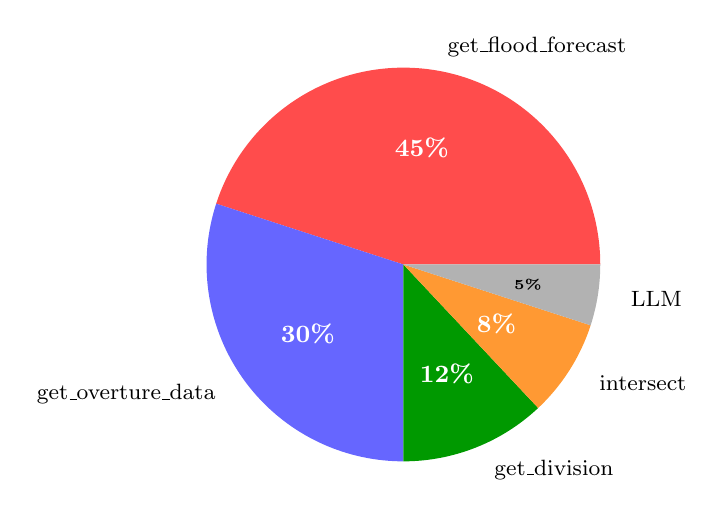
\begin{tikzpicture}
        % Pie chart drawn manually with TikZ
        % Segments: get_flood 45%, get_overture 30%, get_division 12%, intersect 8%, LLM 5%
        % Angles: 162°, 108°, 43.2°, 28.8°, 18°

        % get_flood 45% (0° to 162°) - red
        \fill[red!70] (0,0) -- (0:2.5) arc (0:162:2.5) -- cycle;
        \node[font=\small\bfseries, white] at (81:1.5) {45\%};
        \node[font=\footnotesize, anchor=west] at (81:2.8) {get\_flood\_forecast};

        % get_overture 30% (162° to 270°) - blue
        \fill[blue!60] (0,0) -- (162:2.5) arc (162:270:2.5) -- cycle;
        \node[font=\small\bfseries, white] at (216:1.5) {30\%};
        \node[font=\footnotesize, anchor=east] at (216:2.8) {get\_overture\_data};

        % get_division 12% (270° to 313.2°) - green
        \fill[green!60!black] (0,0) -- (270:2.5) arc (270:313.2:2.5) -- cycle;
        \node[font=\small\bfseries, white] at (291.6:1.5) {12\%};
        \node[font=\footnotesize, anchor=west] at (291.6:2.8) {get\_division};

        % intersect 8% (313.2° to 342°) - orange
        \fill[orange!80] (0,0) -- (313.2:2.5) arc (313.2:342:2.5) -- cycle;
        \node[font=\small\bfseries, white] at (327.6:1.4) {8\%};
        \node[font=\footnotesize, anchor=west] at (327.6:2.8) {intersect};

        % LLM reasoning 5% (342° to 360°) - gray
        \fill[gray!60] (0,0) -- (342:2.5) arc (342:360:2.5) -- cycle;
        \node[font=\tiny\bfseries] at (351:1.6) {5\%};
        \node[font=\footnotesize, anchor=west] at (351:2.8) {LLM};
    \end{tikzpicture}
    \caption{Rozkład czasu wykonania między narzędziami (opracowanie własne)}
    \label{fig:time_distribution}
\end{figure}

Największy udział w~czasie wykonania mają:
\begin{enumerate}
    \item pobieranie danych GloFAS (45\%) -- transfer plików GeoTIFF z~serwera Copernicus,
    \item pobieranie danych Overture (30\%) -- zapytania SQL do MotherDuck, zależne od liczby obiektów,
    \item pobieranie granic (12\%) -- zapytania do Nominatim i~Overpass API,
    \item analiza przestrzenna (8\%) -- zależna od liczby obiektów,
    \item rozumowanie LLM (5\%) -- planowanie i~generowanie odpowiedzi.
\end{enumerate}

\subsection{Podsumowanie testów}

Tabela~\ref{tab:test_summary} przedstawia podsumowanie wyników testów względem wymagań.

\begin{table}[H]
    \centering
    \caption{Podsumowanie wyników testów (opracowanie własne)}
    \begin{tabular}{|l|l|c|c|}
        \hline
        \textbf{Wymaganie} & \textbf{Kryterium} & \textbf{Wynik} & \textbf{Status} \\
        \hline
        RN-01 & Czas odpowiedzi $\leq$ 30~s & 87,5\% $\leq$ 30~s & PASS \\
        \hline
        RN-02 & Interpretacja NL $\geq$ 80\% & 80\% & PASS \\
        \hline
        RF-01--RF-08 & Wymagania funkcjonalne & 93,3\% (14/15) & PASS \\
        \hline
    \end{tabular}
    \label{tab:test_summary}
\end{table}

\textbf{Wnioski z~testów:}
\begin{enumerate}
    \item system spełnia wszystkie wymagania niefunkcjonalne (RN-01, RN-02),
    \item 93,3\% scenariuszy funkcjonalnych zakończonych sukcesem,
    \item wskaźnik interpretacji języka naturalnego (80\%) spełnia wymaganie RN-02,
    \item wąskie gardło wydajności stanowi transfer danych GeoTIFF z~serwera Copernicus (45\% czasu),
    \item główne ograniczenie: czas \texttt{get\_overture\_data} dla dużej liczby obiektów (>100\,000) -- scenariusz Kraków (30,2~s samego zapytania).
\end{enumerate}

